\chapter{Mass conservation in ACLS}
\label{app:IBs_mass_conservation_ACLS}


It was shown in Section \ref{subsec:ch5_direct_measurement_fluxes_IB} that liquid fluxes decrease downstream the injection point in the planes perpendicular to crossflow. Quantifiying the filming fluxes that reach the wall has also shown that actually the total mass flow rate is not conserved, as the addition of the mean perpendicular and filming fluxes up to a given $x$ location downstream injection does not amount to the injected flow: there is liquid loss with the $x$ distance.

The ACLS/AMR methodology was described in $\S$\ref{subsec:ch2_ACLS}. Two sources of mass loss were identified in this numerical strategy: 

\begin{itemize}

	\item \textbf{Flagging the levelset band}. The levelset band needs to be flagged at each iteration in order to define the region where to compute interface features such as signed distance, normals, curvature and reinitialization fluxes \citepColor[janodet_massively_2022]. When encountering cell-size gradients, it has been observed that some liquid structures diffuse in the mesh and dissappear. The amount of liquid lost by this source is quantitied and discussed in this section.
	
	\item \textbf{Mesh adaptation}. Adaptive Mesh Refinement (AMR) is automatically triggered at a reasonable frequency for AMR which is neither too low (adaptation triggered very often, yielding high computational costs) nor too high (adaptation barely happens and the advected interface finds cell size gradients). Nevertheless, regions in the mesh containing small droplets with size close to mesh resolution or which are travelling fast might sometimes be difficult to adapt, and liquid might disappear there when triggering AMR. The quantity of liquid lost in these computational rotuines has not been directly quantified, but can be estimated by substracting the quantity lost by the band flagging to the total volume of levelset in the domain.

\end{itemize}

In order to retrieve the quantity of lost liquid due to band flagging, the $\psi$ function has been clipped before the flagging step is performed. This function is then denoted as $\psi^-$. Then, the  $\psi$ function after flagging is done is also clipped and denoted as $\psi^+$. Therefore, a field determining the spatial and temporal distribution of levelset loss due to band flagging process can be defined as:

\begin{equation}
\label{eq:ch5_LS_loss_delta_psi_field}
\Delta \psi \left( \textbf{x}, t \right) = \psi^- \left( \textbf{x}, t \right)  - \psi^+ \left( \textbf{x}, t \right) 
\end{equation}

where the mass loss regions is defined for values $\Delta \psi \left( \textbf{x}, t \right) > 0$. From the levelset function $\psi$, the amount of liquid volume present in the domain can be obtained at each iteration from Eq. (\ref{eq:liquid_volume_from_levelset_definition}). The $\psi$ field in this expression corresponds to the one after performing the band flagging process, i.e. $\psi^+$, hence the liquid volume at each iteration could be denoted as $V_l^+$. For simplicity reasons, it will be simply denoted as $V_l$ in the graphs that follow. In the same fashion, liquid volume before the band flagging operation can also be obtained with $\psi^-$, which yields then a volume $V_l^-$. From these two quantities, the amount of loss liquid at each time instant $t_i$ due to the band flagging (BF) process can then be easily obtained as their difference:

\begin{equation}
\Delta V_{l,\mathrm{BF}} \left( t_i \right)  = V_l^- \left( t_i \right)  - V_l^+ \left( t_i \right)
\end{equation}

And hence, the total liquid volume loss at one simulation due to the band flagging process can be monitored in time $t$ as follows:

\begin{equation}
\label{eq:ch5_LS_loss_delta_Vl_BF}
\Delta V_{l,\mathrm{BF}}  \left( t \right) = V_l^- \left( t \right)  - V_l^+ \left( t \right) + \int_{t_0}^t \Delta V_{l,\mathrm{BF}} \left( \tau \right) d\tau
\end{equation}

Where $t_0$ is the first time instant at each simulation run. The last integral term has been added so that $\Delta V_l$ represents the accumulated liquid volume lost throughout a run. This quantity can now be added to the total volume at the end of each iteration to provide the liquid volume that would be present at the domain if there was no mass loss due to band flagging, named $V_{l,\mathrm{NF}}$:

\begin{equation}
\label{eq:ch5_liquid_volume_no_flagging}
V_{l,\mathrm{NF}}  \left( t \right) = V_l  \left( t \right) + \Delta V_{l,\mathrm{BF}} \left( t \right)
\end{equation}

Finally, the total amount of liquid volume injected in a simulation run can be quantified with the following expression:

%\begin{equation}
%\label{eq:ch5_liquid_volume_injected}
%V_{l,\mathrm{inj}} \left( t \right) = V_{l,0} + \sum_{i=1}^{N_\mathrm{iter}} \Delta t_i Q_\mathrm{injected}
%\end{equation}

\begin{equation}
\label{eq:ch5_liquid_volume_injected}
V_{l,\mathrm{inj}} \left( t \right) = V_{l,0} + \int_{t_0}^t Q_\mathrm{injected}~d\tau = V_{l,0} + Q_\mathrm{injected}  \left( t - t_0 \right)
\end{equation}

where $V_{l,0}$ is the liquid volume present at the beginning of every simulation run. $V_{l,\mathrm{inj}}$ represents therefore the quantity of liquid volume that would be present in the domain if there was not mass loss of any kind,i.e. neither through levelset band flagging nor to mesh adaptation. Then, the total volume loss can be computed as:

\begin{equation}
\label{eq:ch5_LS_loss_delta_Vl_total}
\Delta V_{l,\mathrm{total}}  \left( t \right)  = V_{l,\mathrm{inj}} \left( t \right) - V_l \left( t \right)
\end{equation}

With Eqs. (\ref{eq:ch5_LS_loss_delta_psi_field}) and (\ref{eq:ch5_LS_loss_delta_Vl_total}), the amount of volume lost can be fully characterized: the former provides an instantaneous field of the location in which liquid disappears due to the band flagging process, and the latter yields the instantaneous amount of levelset loss. Then, the losses due to the band flagging process are calculated with Eq. (\ref{eq:ch5_liquid_volume_no_flagging}). Finally, the difference of Eqs. (\ref{eq:ch5_LS_loss_delta_Vl_total}) and (\ref{eq:ch5_liquid_volume_no_flagging}) provides the mass loss which is not due to the band flagging process, and which is thought to be caused by the AMR process as shown later. This magnitude is denoted as $\Delta V_{l,\mathrm{NBF}}$: 

\begin{equation}
\Delta V_{l,\mathrm{NBF}} = \Delta V_{l,\mathrm{total}} - \Delta V_{l,\mathrm{BF}}
\end{equation}

Evaluation of mass loss is performed in two simulations for the two resolutions of the high Weber case: UG100\_DX20, UG100\_DX10 (see Table \ref{tab:jicf_resolved_simulations_performed},).. Computations are run for a short time ($\Delta t^* = 0.6$) without artificial liquid removal at the end of the domain, otherwise the application of Eqs. (\ref{eq:liquid_volume_from_levelset_definition}) (\ref{eq:ch5_liquid_volume_no_flagging}) would also account for this artificial loss. The parameters from the ACLS methodology that can have an influence on the $\psi$ loss are the interface thickness $\varepsilon$ from Eq. (\ref{eq:ACLS_psi_definition}) and the number of reinitiation steps $N_\mathrm{reinit}$ of the reinitialization equation (\ref{eq:acls_reinit_2017}). These two parameters are tested hereafter with case UG100\_DX20; case UG100\_DX10 is only studied with one configuration to evaluate the influence of interface resolution. The four simulations performed are shown in Table \ref{tab:jicf_simulations_mass_loss_set_levelset_band}, where Case 1 is the baseline case. 

\begin{table}[!h]
\centering
\caption{Simulations performed to evaluate mass loss due to ACLS}
\begin{tabular}{cccc}
\thickhline
\textbf{Case} & $\Delta x_\mathrm{min} ~ [\mu \mathrm{m}]$ & $N_\mathrm{reinit}$ &  $\varepsilon$ \\
\thickhline
1 & 20 & 3 & 0.5 \\
2 & 20 & 6 & 0.5 \\
3 & 10 & 3 & 0.5 \\
4 & 20 & 3 & 0.7 \\
\thickhline
\end{tabular}
\label{tab:jicf_simulations_mass_loss_set_levelset_band}
\end{table}

%\begin{figure}[h!]
%	\centering
%	\includeinkscape[inkscapelatex=false,scale=0.3]{./part2_developments/figures_ch5_resolved_JICF/flow_rates_mass_loss_set_levelset_band/mass_loss_baseline}
%	\caption{Case 1 (baseline)}
%	\label{fig:jicf_mass_loss_baseline}
%\end{figure}
%
%\begin{figure}[h!]
%	\centering
%	\includeinkscape[inkscapelatex=false,scale=0.4]{./part2_developments/figures_ch5_resolved_JICF/flow_rates_mass_loss_set_levelset_band/mass_loss_dx10}
%	\caption{Case 4 (dx10)}
%	\label{fig:jicf_mass_loss_dx10}
%\end{figure}

\begin{figure}[h!]
	\centering
	\includeinkscape[inkscapelatex=false,scale=0.3]{./part2_developments/figures_ch5_resolved_JICF/flow_rates_mass_loss_set_levelset_band/mass_loss_baseline_and_dx10}
	\caption{Regions of mass loss at the end of simulation for (a) case 1 (baseline) and (b) case 3 ($\Delta x_\mathrm{min} = 10~\mu$m).}	\label{fig:jicf_mass_loss_baseline_and_dx10}
\end{figure}

\subsubsection*{Case 1: Baseline }

Figure \ref{fig:jicf_mass_loss_baseline_and_dx10} shows a instantaneous snapshot of the jet. The black field denotes the regions with $\Delta \psi \left( \textbf{x}, t \right) > 0$ for the whole duration of the simulation. Losses are distributed right downstream the jet dense core due to the droplets coming from surface breakup that reach a size of the order of the mesh resolution and disappear (see $\S$\ref{subsec:ch5_breakup_topology}), and also further downstream along the jet as the ligaments from column breakup form small droplets that eventually vanish. The further downstream the injection point, the more liquid is lost, which explains the reduction in mean flow rates with increasing axial distance from Figure \ref{fig:IB_bargraph}. The evolution of the liquid volumes calculated from Eqs. (\ref{eq:liquid_volume_from_levelset_definition}), (\ref{eq:ch5_liquid_volume_injected}) and (\ref{eq:ch5_liquid_volume_injected}) are shown in Figure \ref{fig:JICF_liquid_evolution_loss_due_to_set_levelset_band}a by the black, blue and red lines respectively. The iterations at which mesh adaptation is performed are denoted by the dashed grey lines.  As observed, $V_{l,\mathrm{inj}}$ evolves linearly with time as the injected flow rate is constant. From the early instants of the simulation, the curve given by $V_l$ starts to diverge from $V_{l,\mathrm{inj}}$ due to the mass lost in the band flagging process. On the contrary, the line for $V_{l,\mathrm{NF}}$ follows the same trend as $V_{l,\mathrm{inj}}$ until the first adaptation iteration in the simulation, where a slight mass decrease is observed. As the simulation runs, the $V_{l,\mathrm{NF}}$ line keeps the same slope as $V_{l,\mathrm{inj}}$ but sees step reductions at several AMR iterations. The line $V_l$, on the other hand, suffers volume losses at certain AMR iterations but also among adaptation iterations: in particular, a strong gradual decrease has been captured between the adaptation iterations 4 and 5. This demonstrates that the losses not due to band flagging are observed only at the adaptation iterations, while the ones due to band flagging are also present outside the adaptation procedure. 

The mass losses at the end of the run are shown in Figure \ref{fig:JICF_liquid_evolution_loss_due_to_set_levelset_band}.: graph (a) shows the absolute losses, while graph (b) shows the pertentual contribution of the each source to the total volume loss. As observed from Figure \ref{fig:JICF_liquid_evolution_loss_due_to_set_levelset_band}(b), most of the liquid suppression is caused by the band flagging process ($88~\%$) while only a small percentage happens outside this routine. This demonstrates that, with the parameters from case 1, the band flagging is the main source of liquid loss in the simulations.

\subsubsection*{Case 2: Effect of $N_\mathrm{reinit}$}



The effect of the number steps to perform the steps of the levelset reinitialization equation (\ref{eq:acls_reinit_2017}), $N_\mathrm{reinit}$, is increased increased from 3 to 6. Increasing the number of steps helps to better maintain the hyperbolic tangent profile of the levelset, to avoid numerical and to reduce spurious oscillations around the interface in flows where the interface is highly deformed \citepColor[mccaslin_localized_2014], as it is the case of the JICF operating conditions studied in this chapter. Consequently, the interface location $\psi = 0.5$ is better determined and the levelset transport is more accurate. Figure \ref{fig:JICF_liquid_losses_bar_graph}b shows that the $V_l$ curve gets closer to the $V_{l,\mathrm{NF}}$ for all the simulation; in other words, the amount of loss $\Delta V_{l,\mathrm{BF}}$ is reduced. The absolute amount of liquid loss $\Delta V_l$ as given in Figure \ref{fig:JICF_liquid_losses_bar_graph}a is reduced with respect to Case 1, and the percentual contribution of the band flagging to the total loss, given in Figure \ref{fig:JICF_liquid_losses_bar_graph}b, is also reduced: $35~\%$ for $\Delta V_{l,\mathrm{BF}}$ with respect to $65~\%$ obtained for $\Delta V_{l,\mathrm{NBF}}$. It is therefore demonstrated that increasing $N_\mathrm{reinit}$ has a positive effect on mass conservation.


\subsubsection*{Case 3: Effect of $\Delta x_\mathrm{min}$}

Figure \ref{fig:jicf_mass_loss_baseline_and_dx10}b shows an instantaneous snapshot at the end of the simulaton performed with $\Delta x_\mathrm{min} = 10~\mu$m. It is seen that liquid disappearance is more distributed in space than Case 1, which is due to a higher amount of droplets generated by surface and column breakup with a size close to the mesh resolution. At a first glance at the figure, it might seem that the total amount of liquid lost is larger than for case 1: nevertheless, Figure \ref{fig:JICF_liquid_losses_bar_graph}a shows that the total volume loss is in fact of the same order than in Case 1, while the percentual contribution of $\Delta V_{l,\mathrm{BF}}$ is lower than for Case 1 ($78~\%$ with respect to $88~\%$) as given in Figure  \ref{fig:JICF_liquid_losses_bar_graph}b. Effectively, by increasing the mesh resolution from $\Delta x_\mathrm{min}$ = 20 to 10 $\mu$m, the droplets disappearing have a characteristic size of the order of this value and therefore, each individual droplet contains less volume than one droplet disappearing with a size of 20 $\mu$m. Even if there are more droplets disappearing, the total volume being removed by band flagging is lower than in Case 1. There is on the other hand, according to Figure \ref{fig:JICF_liquid_losses_bar_graph}a, an increase in the absolute loss produced outside the band flagging process. by looking at Figure \ref{fig:JICF_liquid_evolution_loss_due_to_set_levelset_band}c, one can see that the reductions in $V_{l,NF}$ also occur during the adaptation iterations. The increase in $\Delta V_{l,\mathrm{NBF}}$ could be due to the fact that by reducing the interface cell size, the adaptation process needs to locate more cells around the interface and finds more difficulties to adapt its neighbouring elements within the levelset band so that their size increases progressively from $\Delta x_\mathrm{min}$ to the baseline mesh resolution. This will also suppose an important increase in the cost of the simulations, as it will be later shown in $\S$\ref{subsec:ch5_computational_performances}. Nevertheless, Figure \ref{fig:JICF_liquid_evolution_loss_due_to_set_levelset_band}c shows that, as in Case 1, the mass loss in the AMR process does not occur at every adaptation iteration but only at a few of them, and also that more AMR iterations have been performed in Case 3 than in Case 1 (for the same time period simulated). If the same number of AMR iterations had been performed, the value of $\Delta V_{l,\mathrm{NBF}}$ might be different: however, the frequency of AMR iterations is calculated automatically by Eq. (\ref{eq:ch2_N_iter_adapt_AMR}) and its possible influence has not been addressed in this study. 




%This graph also displays a larger number of AMR iterations than the other three graphs, being the time period simulated equivalent in all cases. The number of simulation iterations among two AMR iterations is calculated according to Eq. (\ref{eq:ch2_N_iter_adapt_AMR}), which as seen depends on $N_p$, $CFL$,

\subsubsection*{Case 4: Effect of $\varepsilon$}

Finally, the effect of the levelset profile thickness $\epsilon$ is tested by modifying its value from 0.5 (case 1) to 0.7. An increase in $\epsilon$ supposes a wider band region and a more diffuse levelset profile. A decrease from 0.5 to 0.3 was also tested and showed no significant differences with the losses obtained for the former one, therefore it has not been reported in this document. As observed in Figures \ref{fig:JICF_liquid_evolution_loss_due_to_set_levelset_band},
and \ref{fig:JICF_liquid_losses_bar_graph}a the effect of increasing $\varepsilon$ is catastrophic: the amount of volume lost by the band flagging process is huge, and the volume lost during the AMR iterations has also widely increased. For the timespan simulated, the total volume lost adds up to almost 0.25 mm$^3$ compare to less than 0.02 mm$^3$ in the rest of the cases. The relative losses in Figure \ref{fig:JICF_liquid_losses_bar_graph}b do not show a big difference with respect to Cases 1 and 3 however: increasing $\varepsilon$ has a negative effect on both sources of volume loss. \\




\begin{figure}[ht]
\flushleft
\begin{subfigure}[b]{0.45\textwidth}
	\centering
   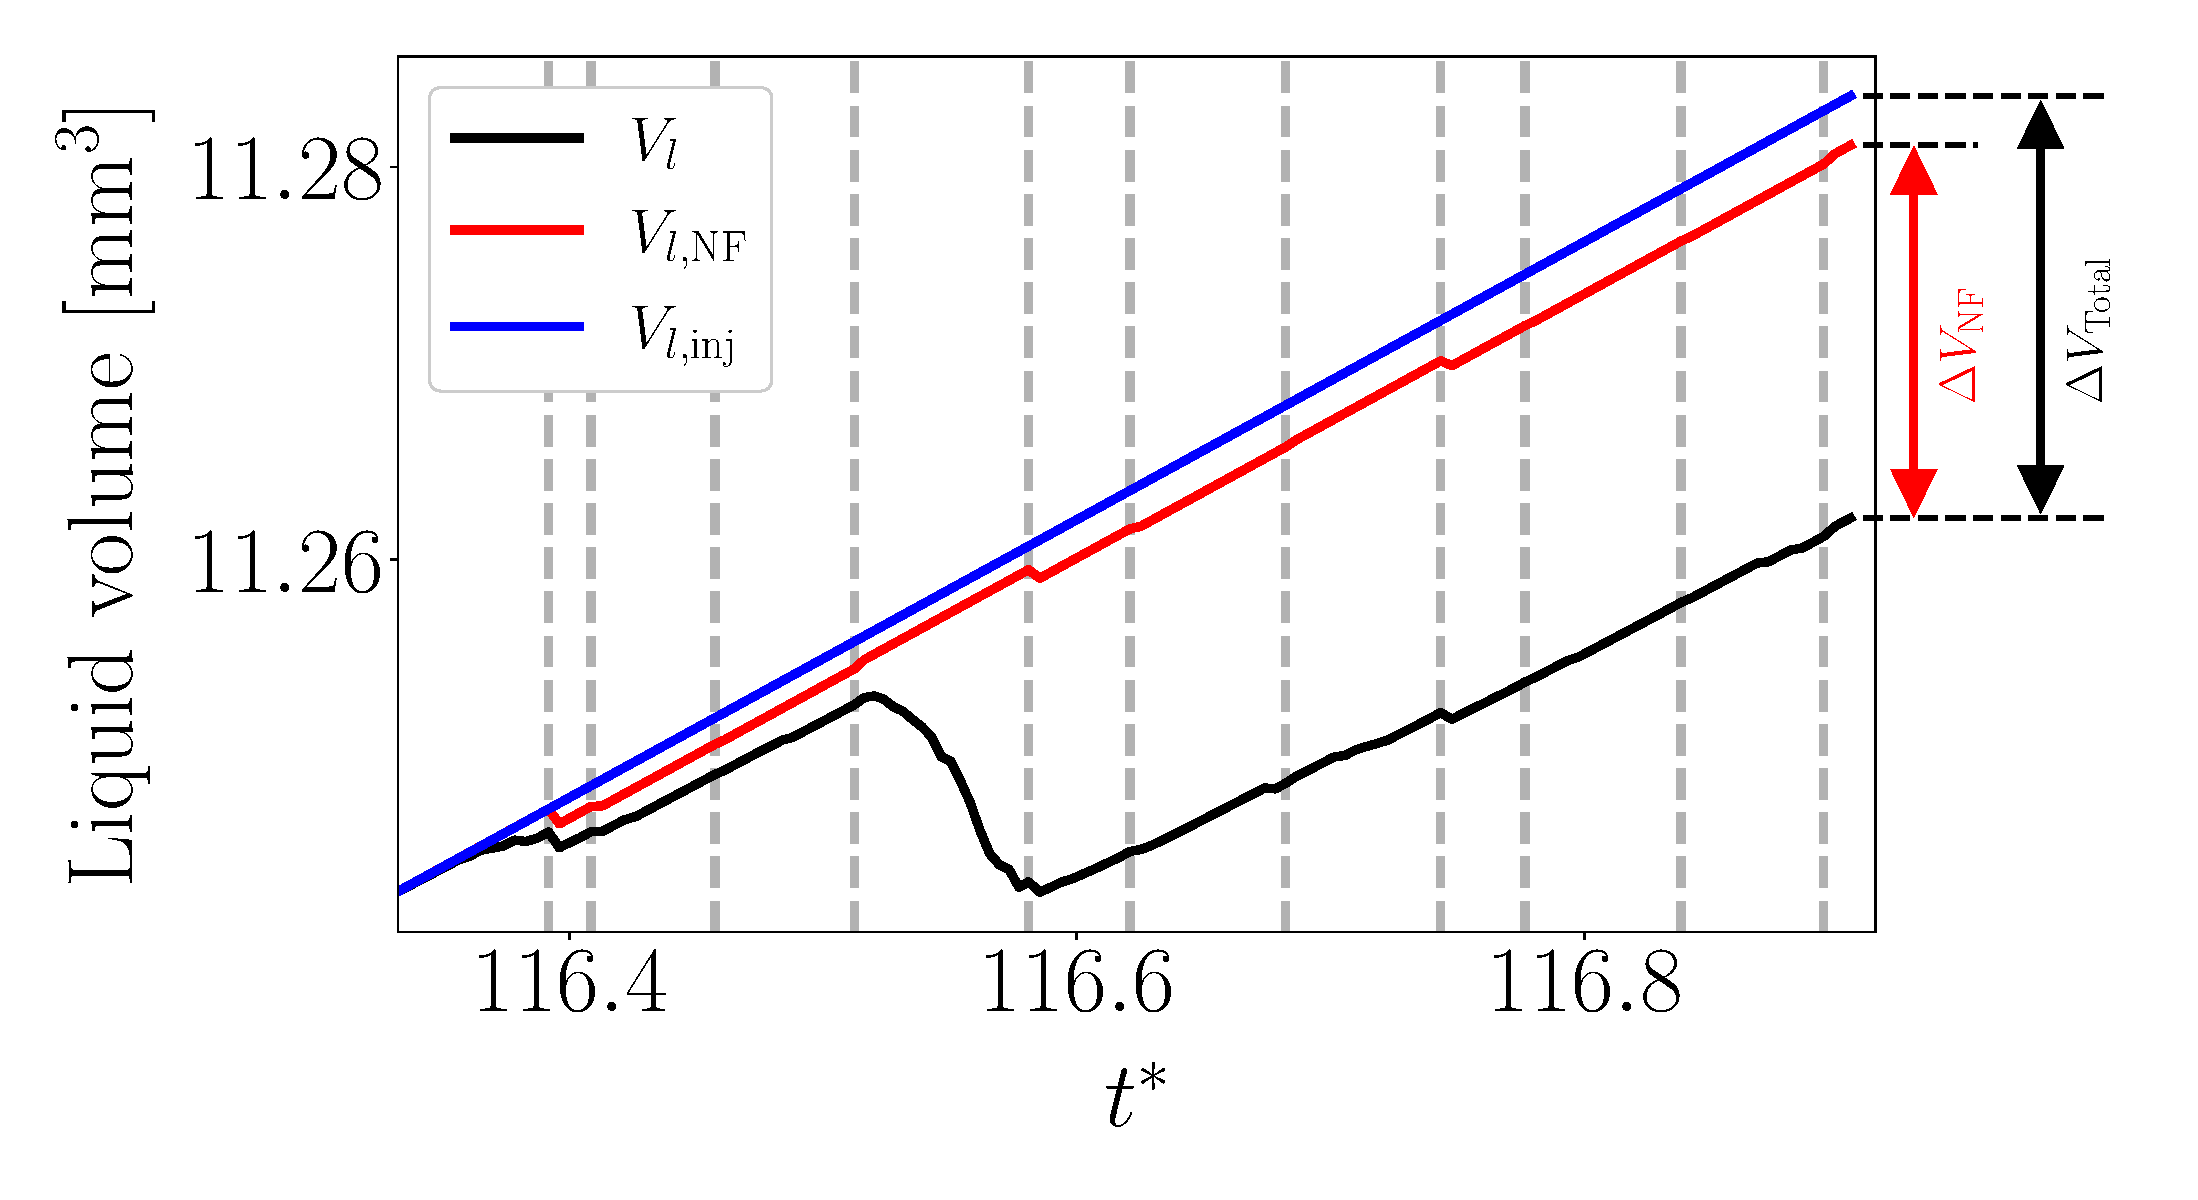
\includegraphics[scale=0.24]{./part2_developments/figures_ch5_resolved_JICF/flow_rates_mass_loss_set_levelset_band/vl_loss_case_baseline}
   \vspace*{-0.2in}
   \caption{Case 1: Baseline}
   %\label{fig:JICF_nelem_increase_all_t} 
\end{subfigure}
\hfill
\begin{subfigure}[b]{0.45\textwidth}
	\centering
   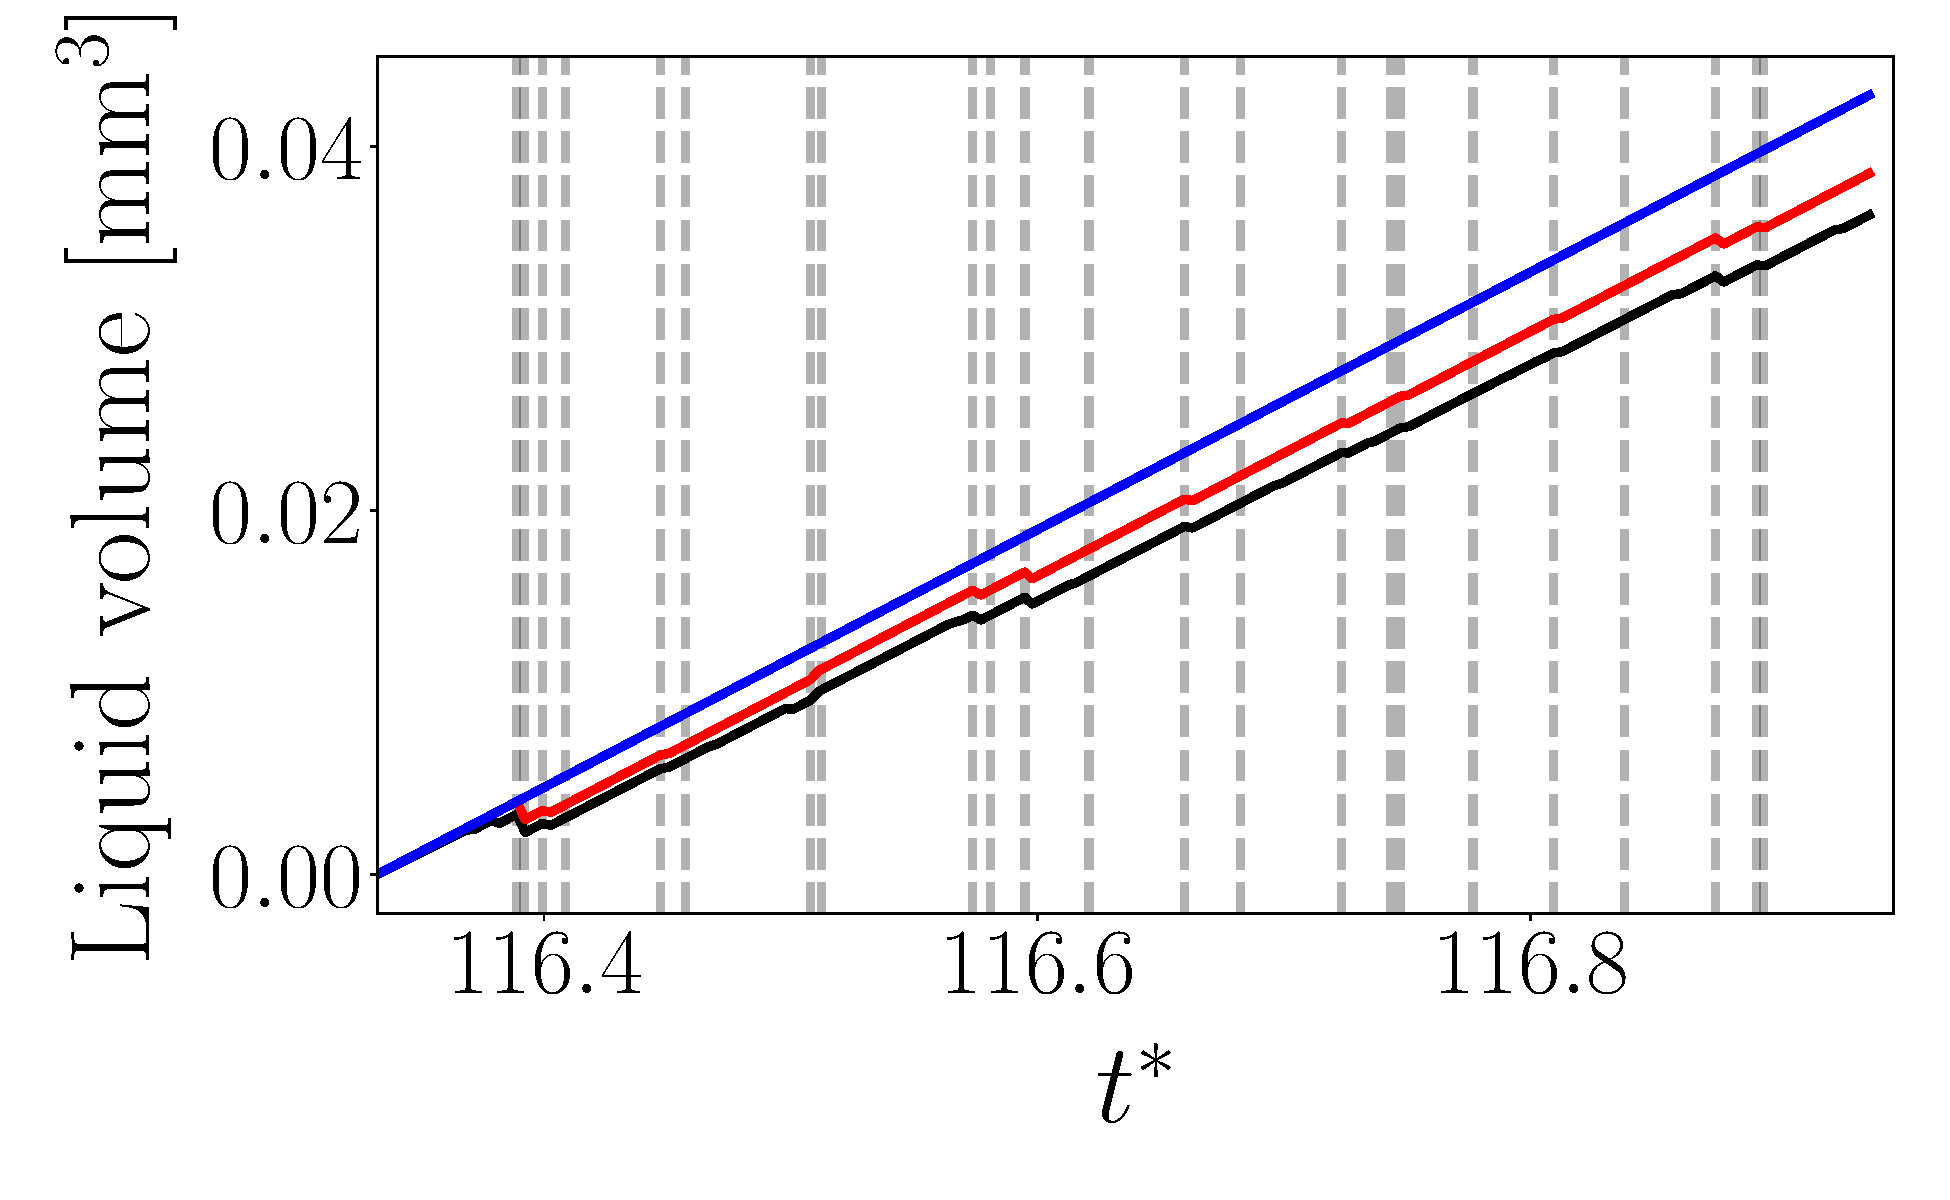
\includegraphics[scale=0.24]{./part2_developments/figures_ch5_resolved_JICF/flow_rates_mass_loss_set_levelset_band/vl_loss_case_Nsteps}
   \vspace*{-0.2in}
   \caption{Case 2: $N_\mathrm{Reinit} = 6$.}
   %\label{fig:JICF_nelem_increase_t_0_to_2}
\end{subfigure}

\vskip\baselineskip

\begin{subfigure}[b]{0.45\textwidth}
	\flushleft
   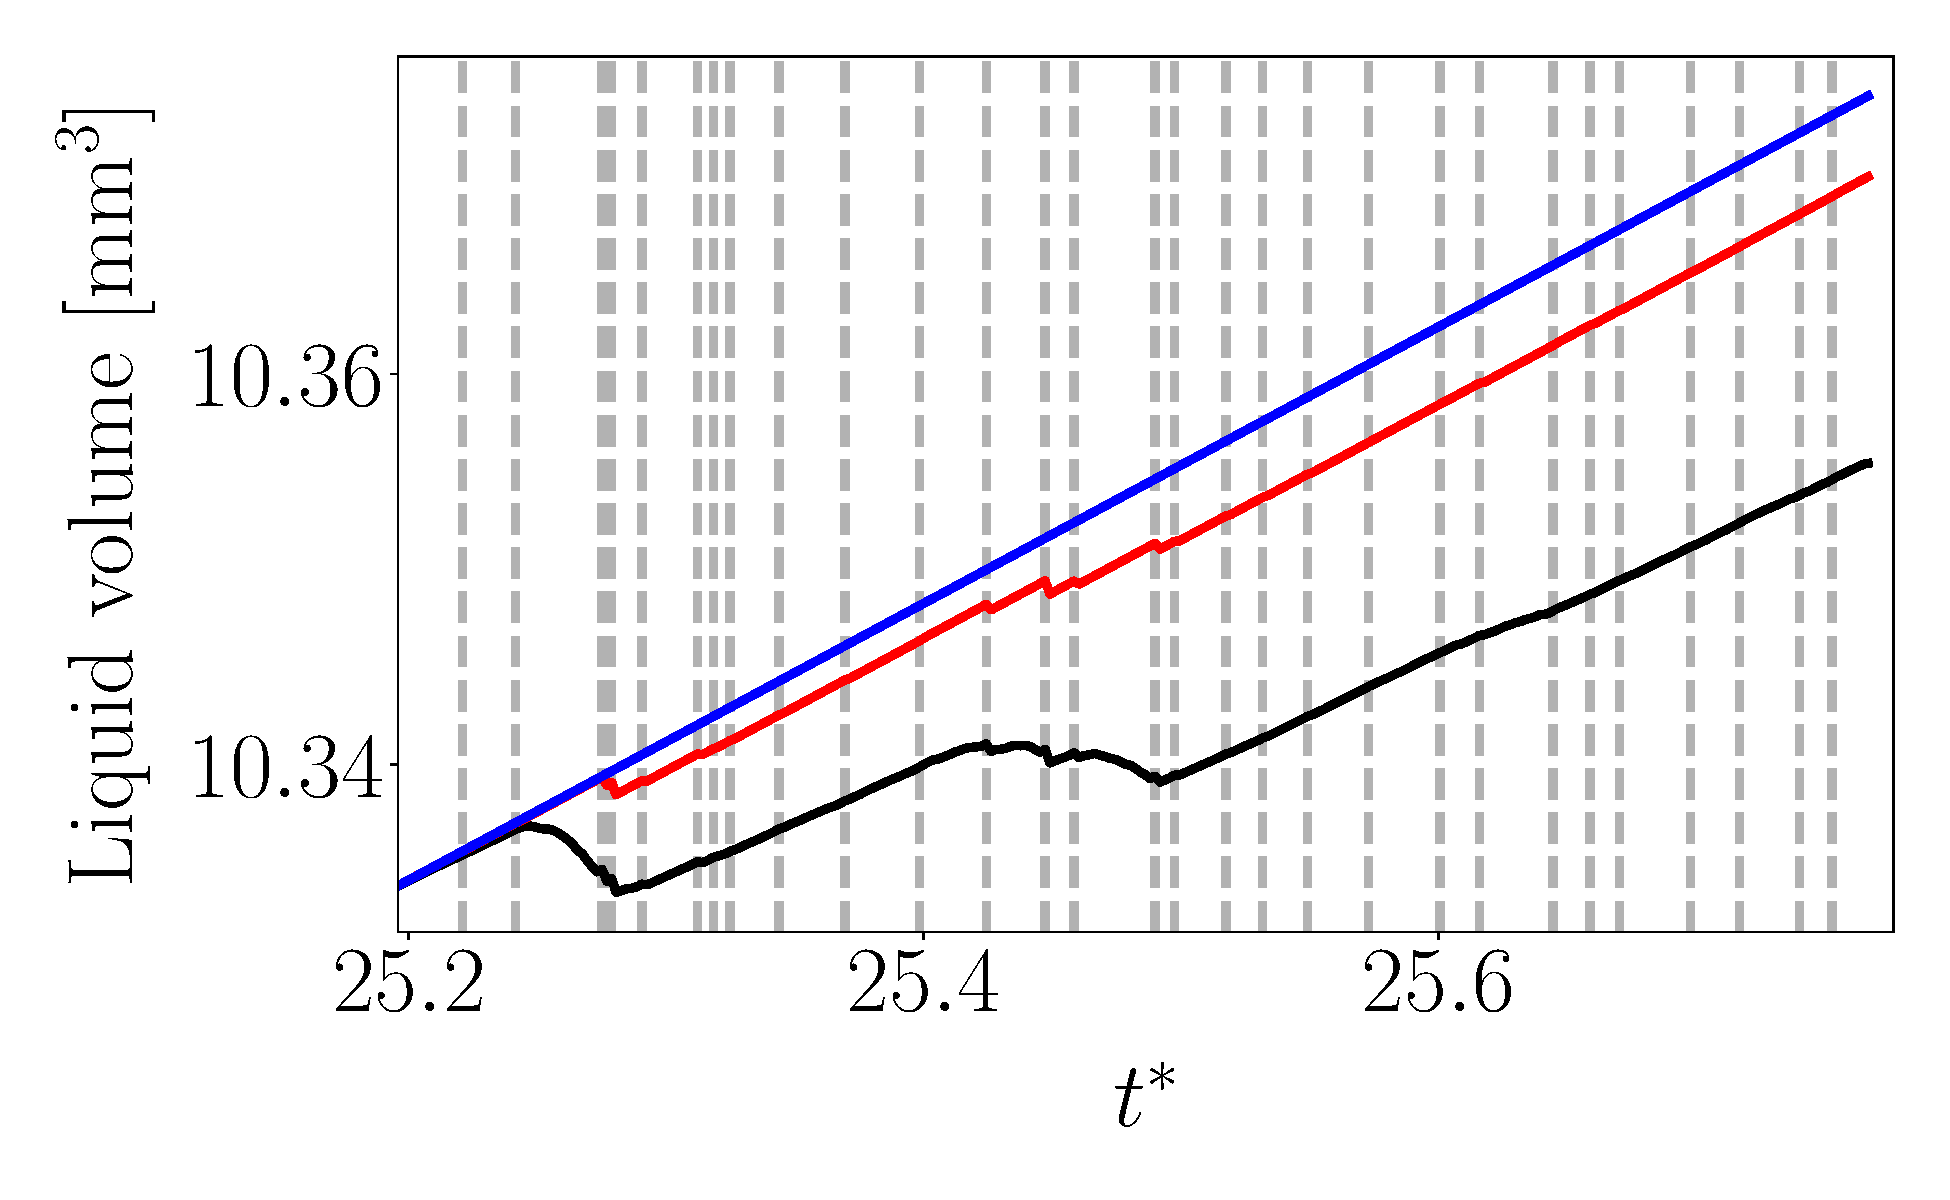
\includegraphics[scale=0.24]{./part2_developments/figures_ch5_resolved_JICF/flow_rates_mass_loss_set_levelset_band/vl_loss_case_dx10}
   \vspace*{-0.2in}
   \caption{Case 3: $\Delta x_\mathrm{min} = 10~\mu$m.}
   %\label{fig:JICF_nelem_increase_all_t} 
\end{subfigure}
\hfill
\begin{subfigure}[b]{0.45\textwidth}
	\centering
   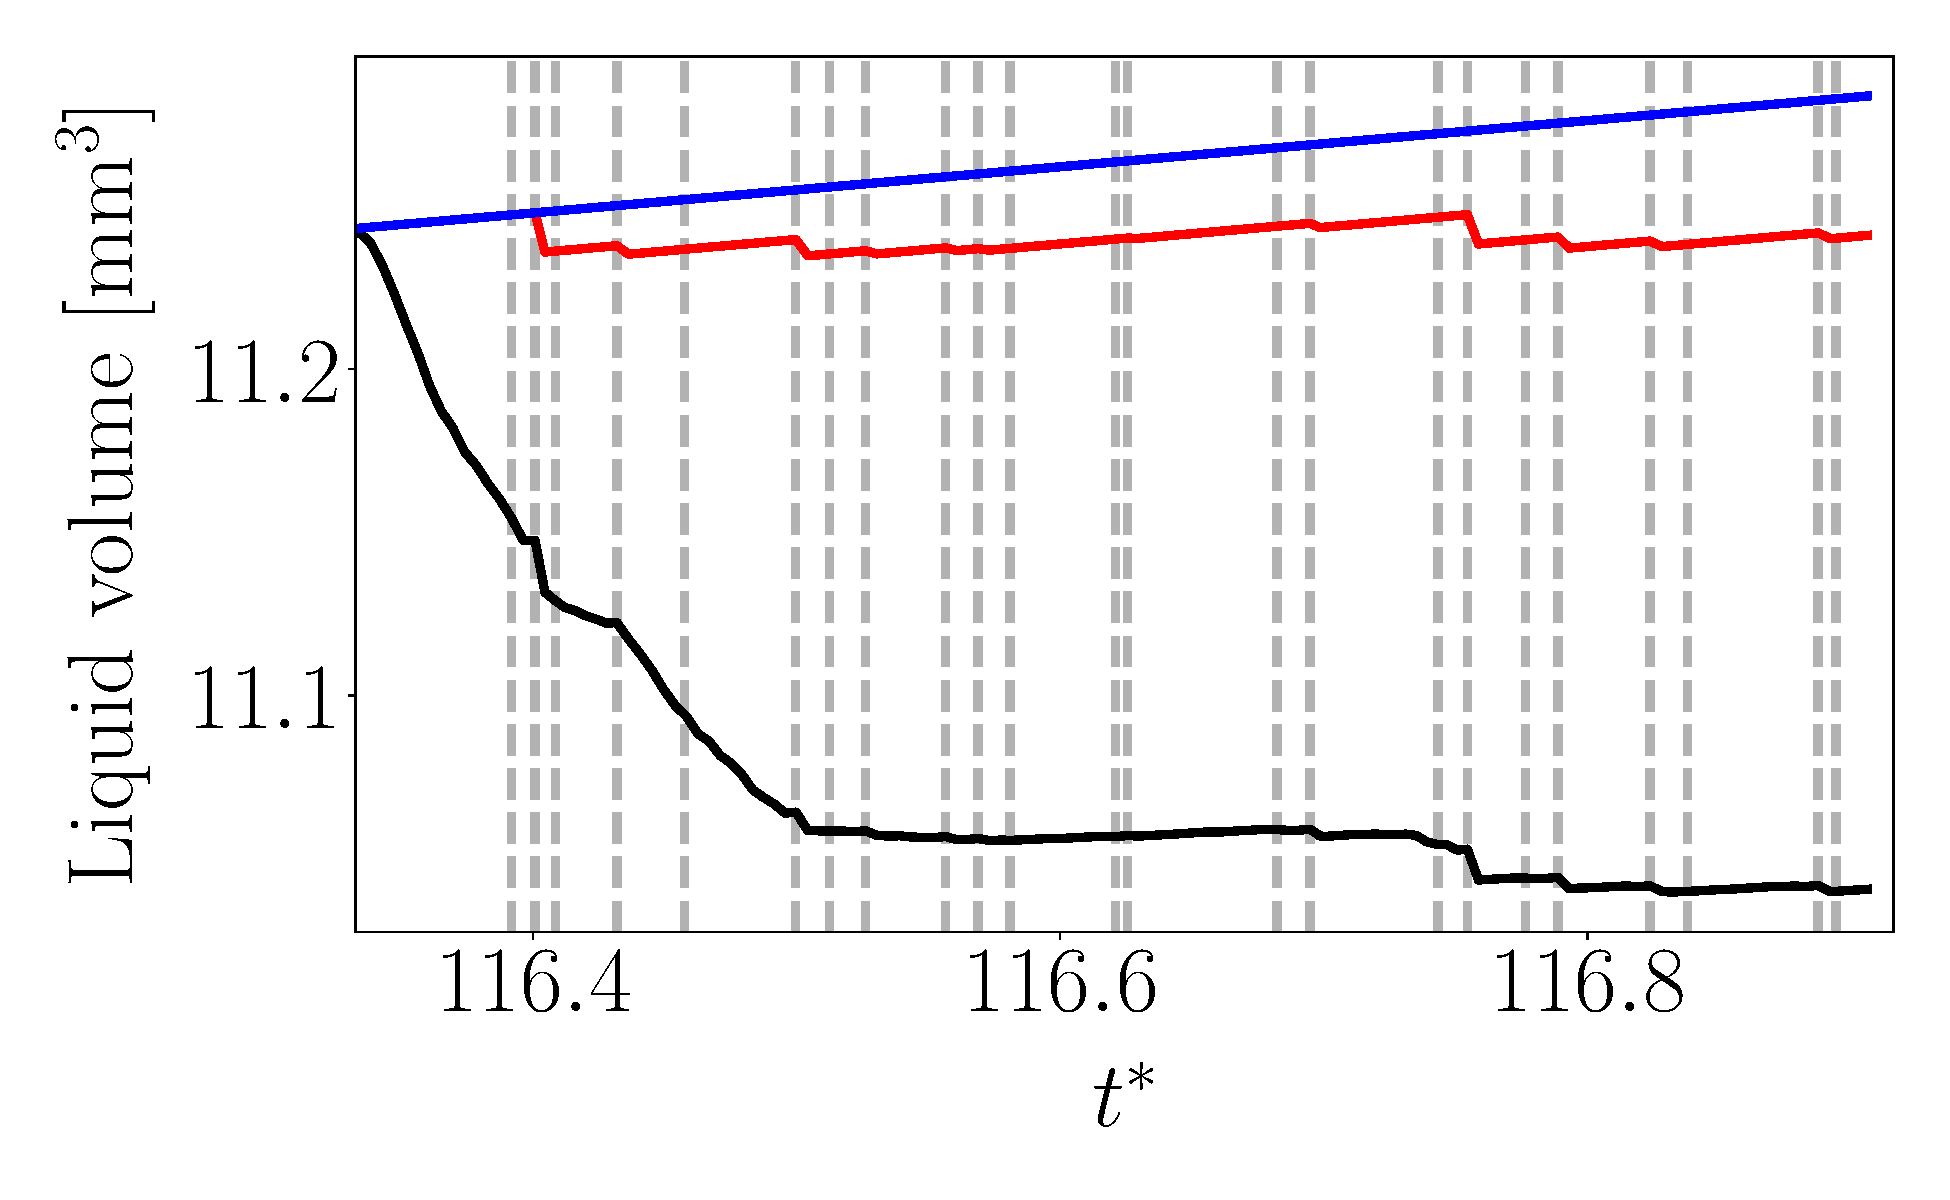
\includegraphics[scale=0.24]{./part2_developments/figures_ch5_resolved_JICF/flow_rates_mass_loss_set_levelset_band/vl_loss_case_epsilon}
   \vspace*{-0.2in}
   \caption{Case 4: $\varepsilon = 0.7$.}
   %\label{fig:JICF_nelem_increase_t_0_to_2}
\end{subfigure}


   \caption[Evolution of liquid volumes]{Evolution of liquid volumes for cases 1 to 4 from Table \ref{tab:jicf_simulations_mass_loss_set_levelset_band}. The dashed grey lines indicate the iterations of adaptation for each case. In all cases the liquid volume present at the initialization of the runs has been substracted from all the curves, in order to the comparison among cases}
\label{fig:JICF_liquid_evolution_loss_due_to_set_levelset_band}
\end{figure}


These simulations have shown that the band flagging process in the ACLS/AMR simulations contributes to the liquid volume loss that causes reductions in the liquid flow rates downstream the injection point. These losses can be reduced by increasing the number of reinitialization steps $N_\mathrm{reinit}$ of the levelset equation. An increase in the levelset thickness $\varepsilon$ has shown to have a detrimental effect on the volume loss. Therefore, the optimal configuration which reduces mass loss has been found for $N_\mathrm{reinit} = 6$, $\varepsilon = 0.5$: all the simulations reported in Chapter \ref{ch5:jicf_resolved_simulations} were performed with these values.




\begin{figure}[ht]
\centering
\begin{subfigure}[b]{0.45\textwidth}
	\centering
   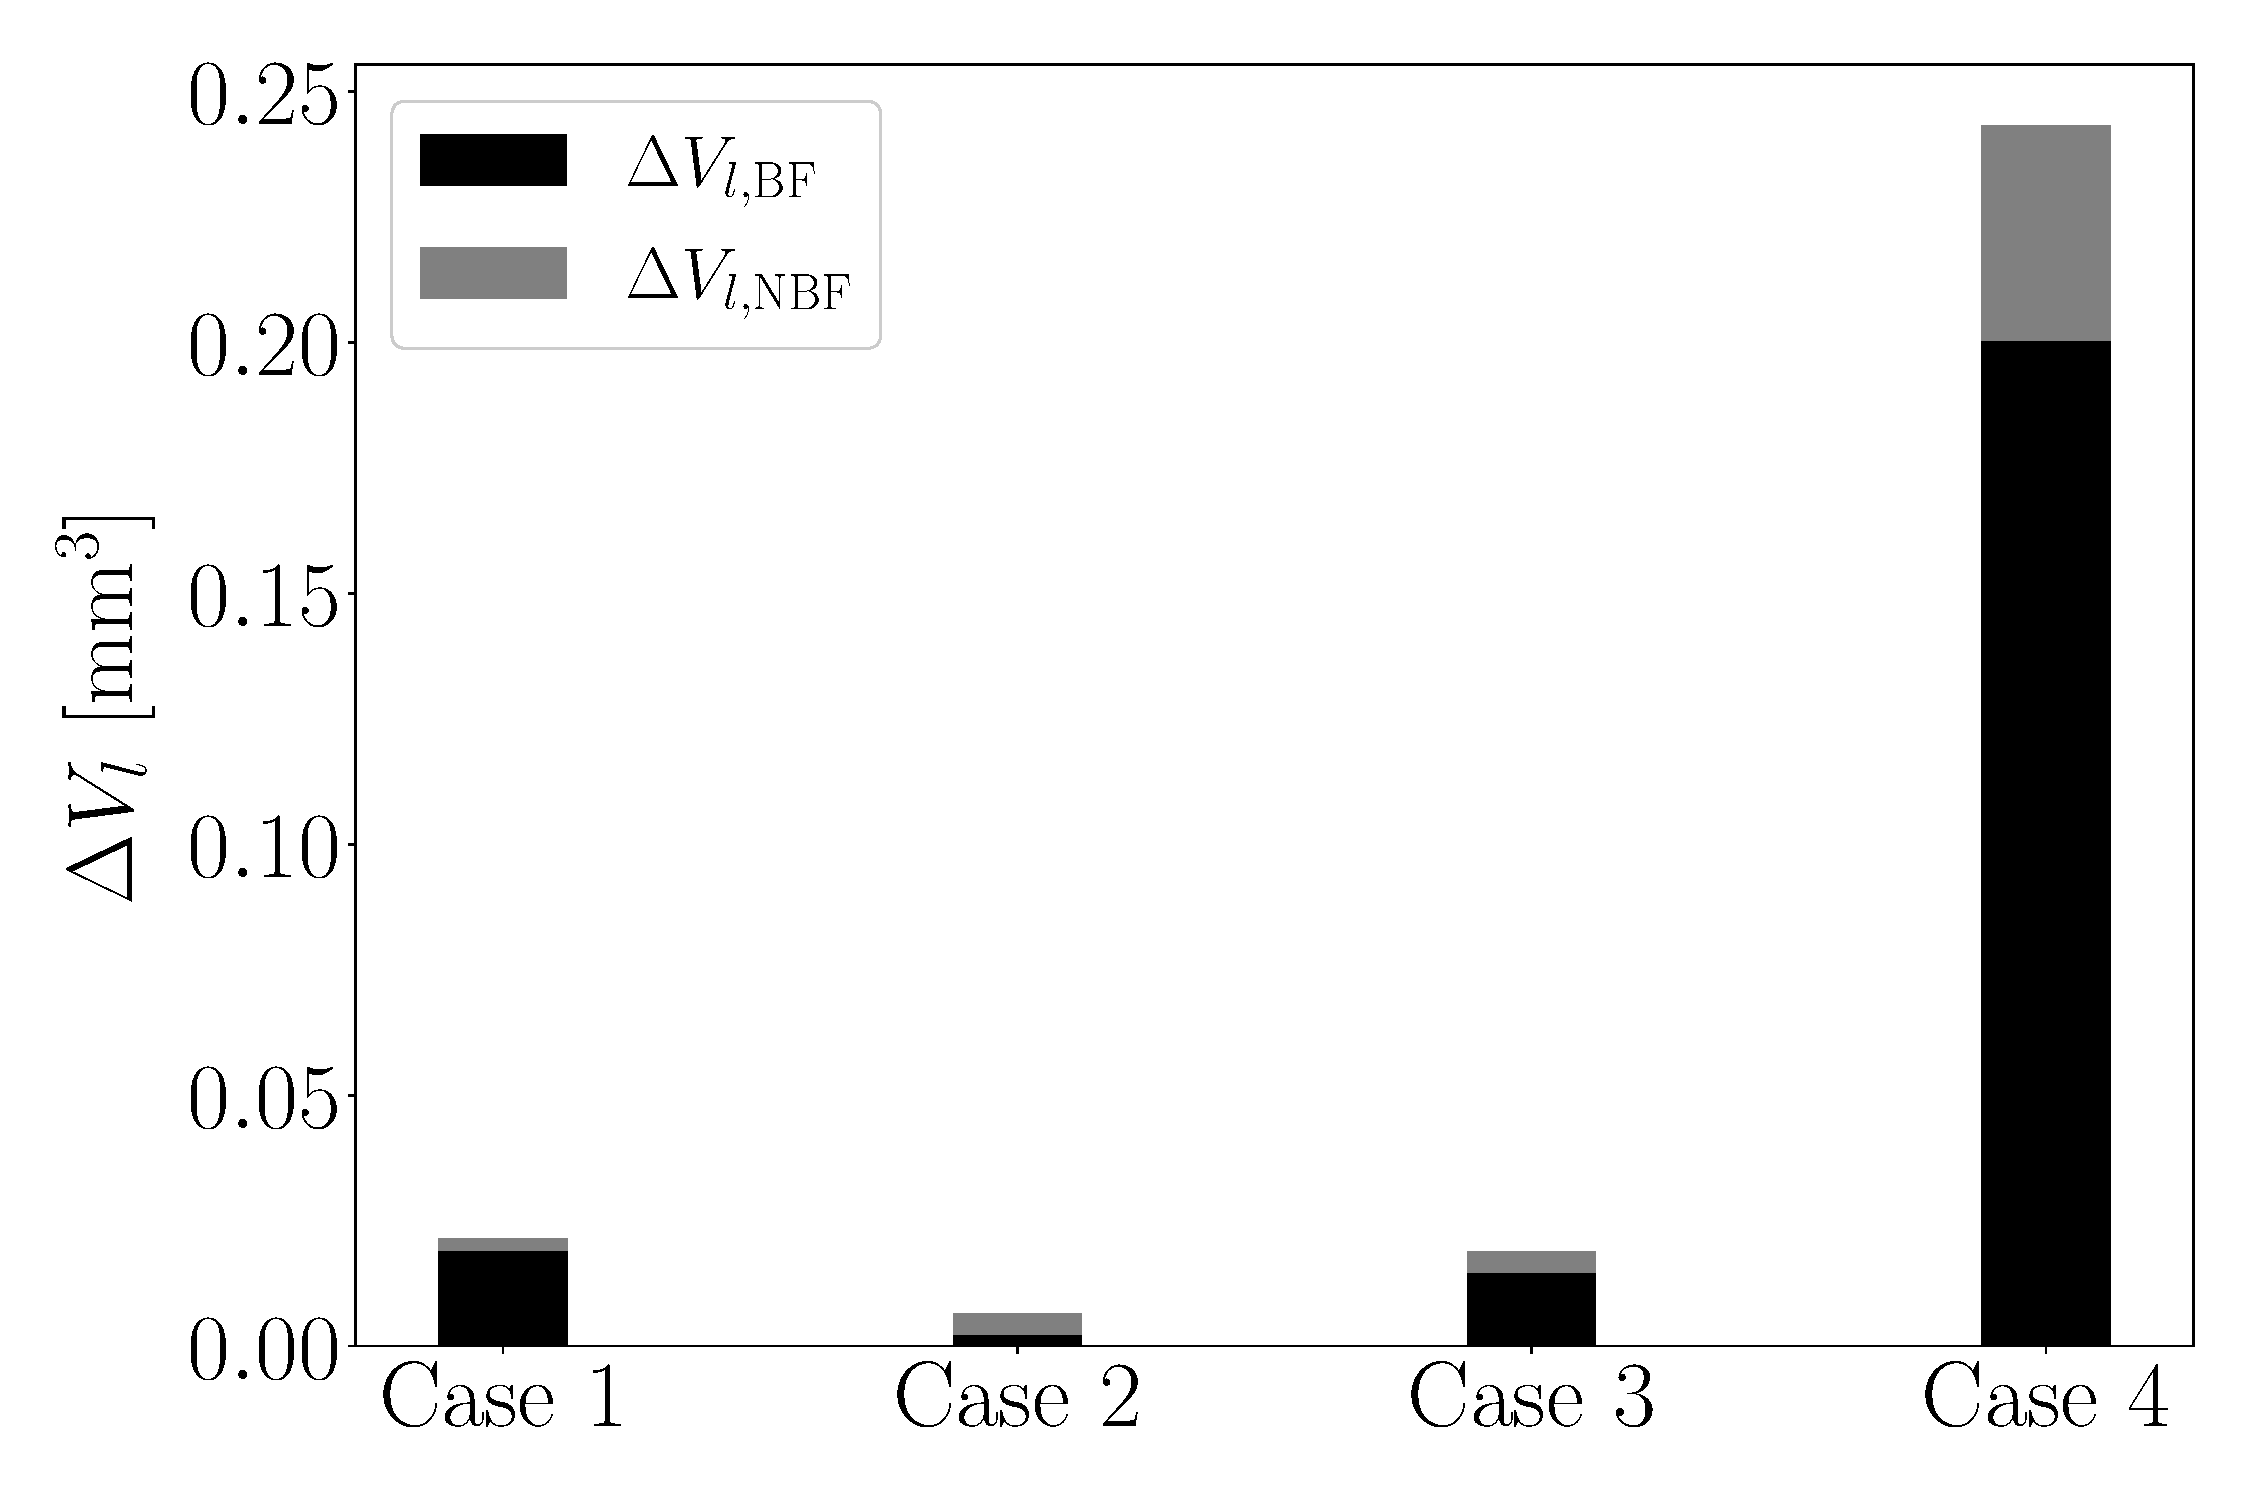
\includegraphics[scale=0.2]{./part2_developments/figures_ch5_resolved_JICF/flow_rates_mass_loss_set_levelset_band/bar_graph_dv_l}
   \vspace*{-0.2in}
   \caption{Absolute volume losses from simulations.}
   %\label{fig:JICF_nelem_increase_all_t} 
\end{subfigure}
\hfill
\begin{subfigure}[b]{0.45\textwidth}
	\centering
   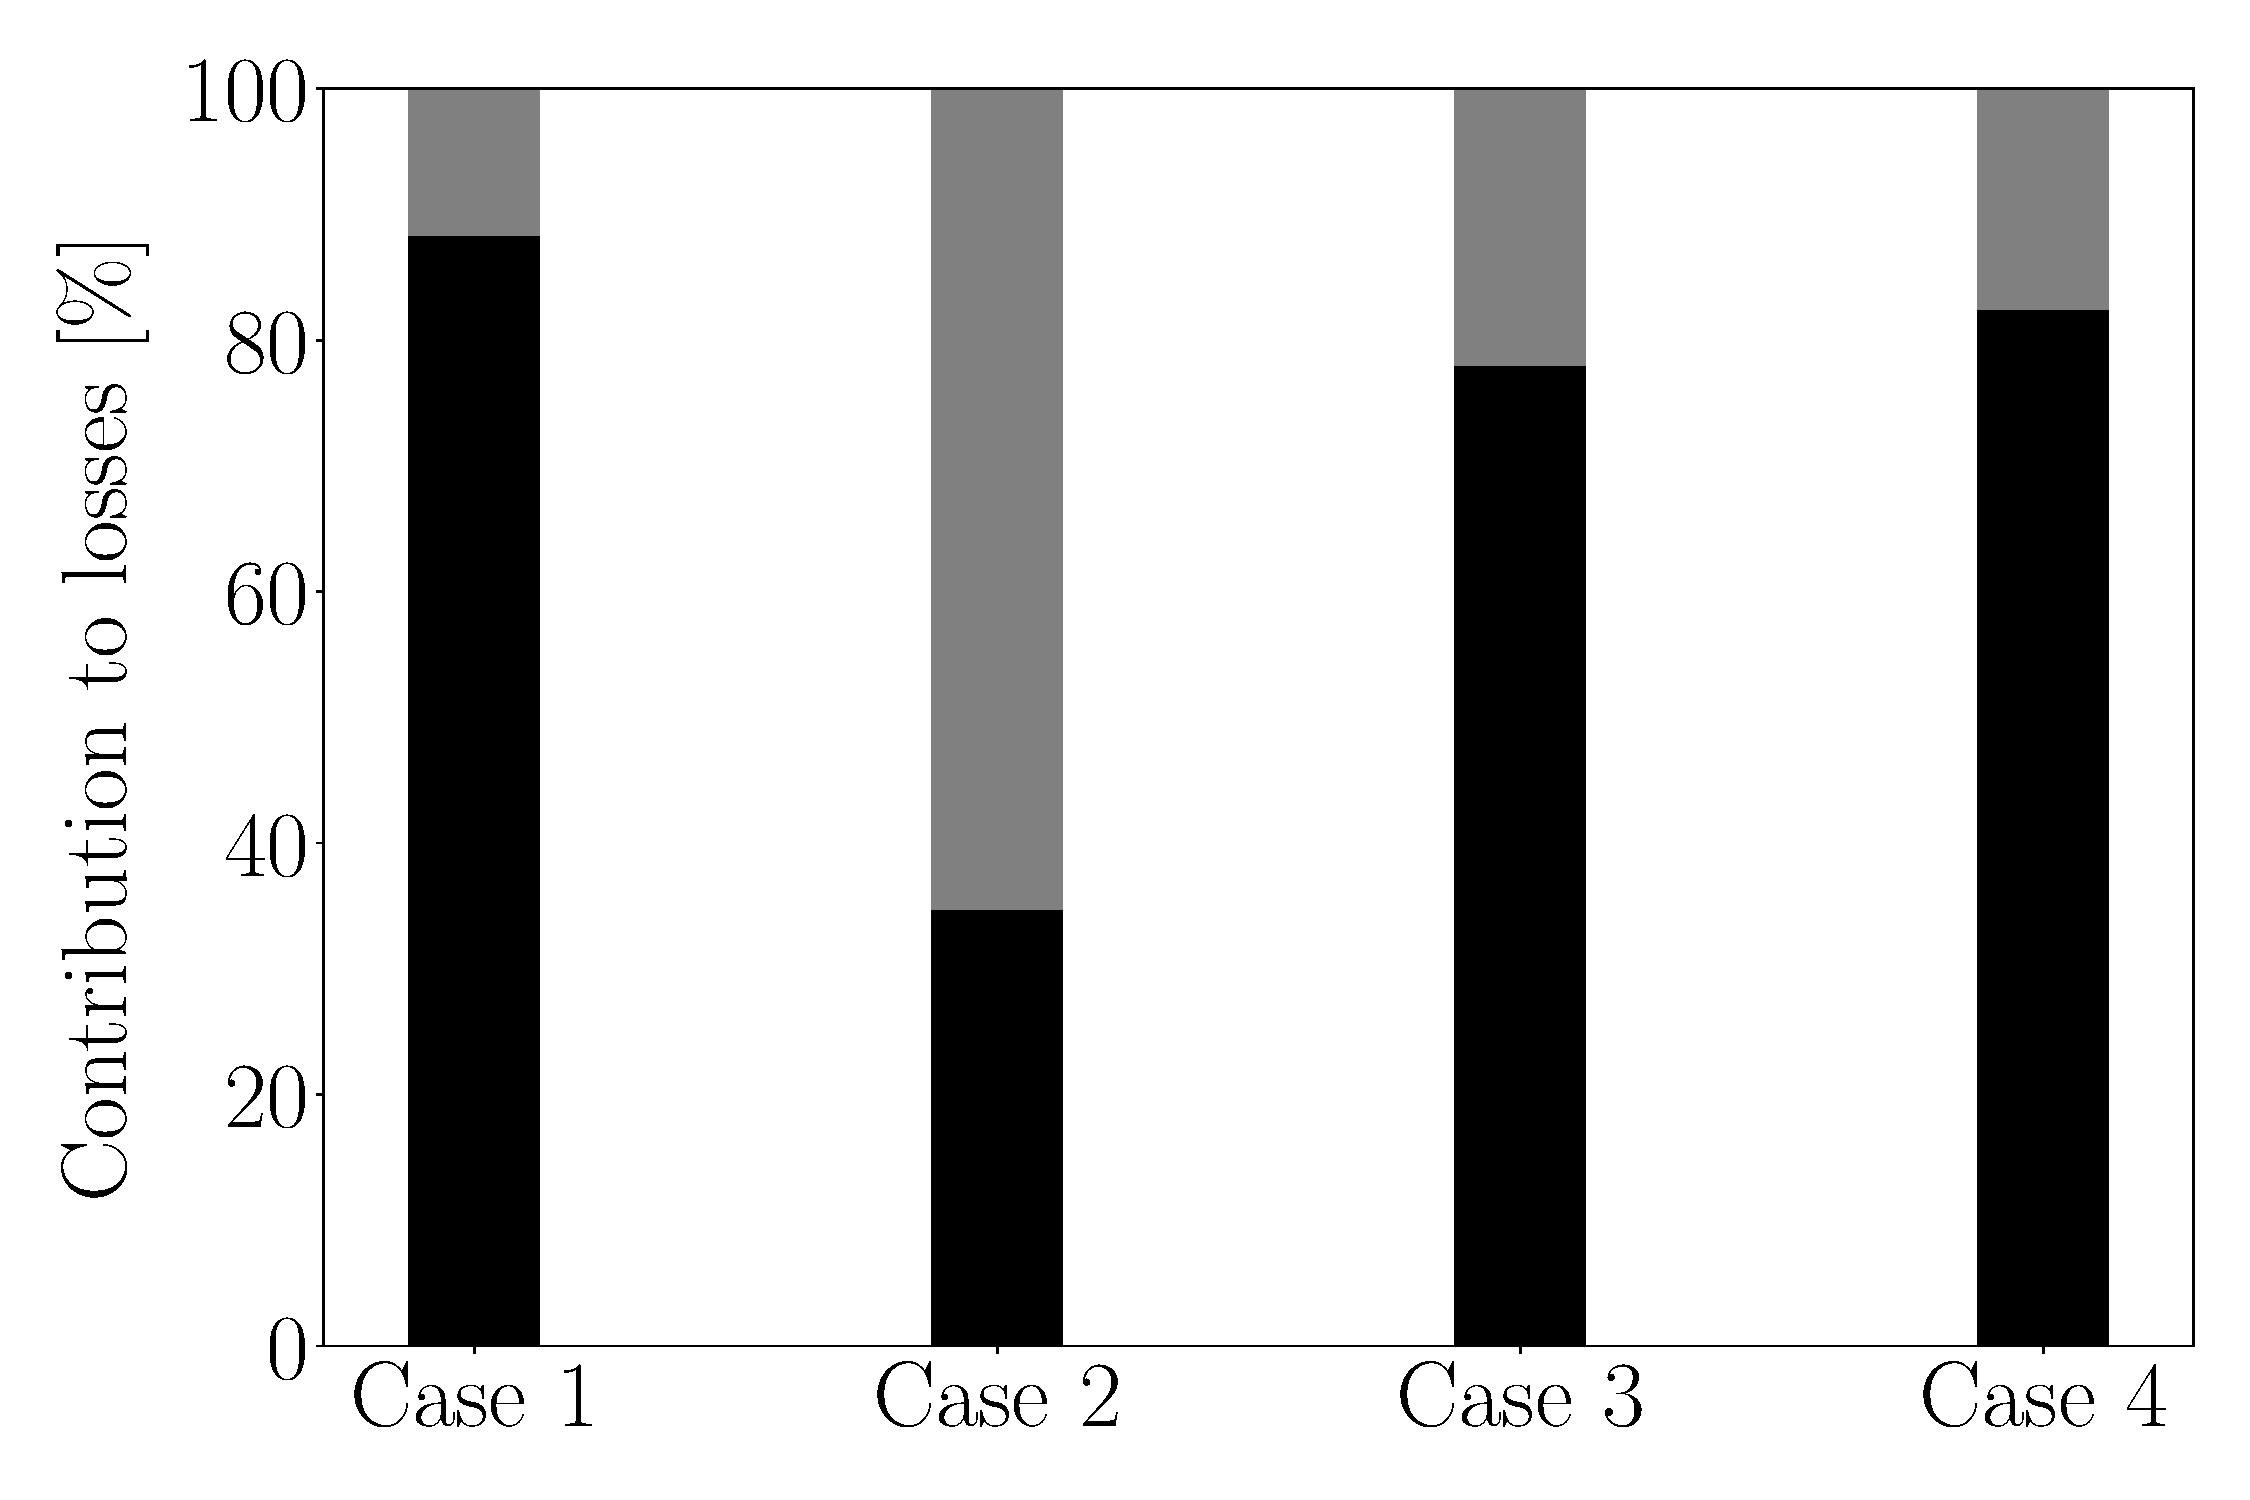
\includegraphics[scale=0.2]{./part2_developments/figures_ch5_resolved_JICF/flow_rates_mass_loss_set_levelset_band/bar_graph_losses_percentage}
   \vspace*{-0.2in}
   \caption{Percentual contribution to total volume loss.}
   %\label{fig:JICF_nelem_increase_t_0_to_2}
\end{subfigure}

   \caption{Liquid volume loss at the end of each run and its contributions}
\label{fig:JICF_liquid_losses_bar_graph}
\end{figure}

